%%%%%%%%%%%%%%%%%%%%%%%%%%%%%%%%%%%%%
\chapter{函数与优化}

在数学中,\textcolor{main}{\bf 函数}是一个基本但强大的工具,它简单地将每一个输入值映射到一个输出值。你可以将它想象为一个机器:你放进一个数(输入),它便会给你另一个数(输出)。

接下来我们将探讨\textcolor{main}{\bf 优化}的概念,它涉及到一个目标函数的最大化或最小化过程,帮助我们在可能的解决方案中找到“最优”的一种。在现实生活中,这可以是找到最省钱的购物清单,或是找到最快的到达目的地的路线。

在本章中,我们将初步探讨函数和优化的基本理论,为你打开一扇理解和掌握这两个强大工具的大门,从而在实际应用中找到最佳的解决方案。

\section{函数的概念和性质}
\subsection{函数的定义}

\begin{note}
    函数是一种数学关系,它将一个集合的元素映射到另一个集合的元素。
\end{note}

\begin{definition}[函数]
给定两个\textcolor{red}{实数集} $D$ 和 $M$, 若有\textcolor{red}{对应法则} $f$, 使对 $D$ 内每一个数 $x$,都有\textcolor{red}{唯一}的一个数 $y \in M$ 与它相对应,则称 $f$ 是定义在数集 $D$上的\textcolor{third}{\bf 函数},记作
\begin{equation}
\begin{aligned}
    f:D & \rightarrow M, \\
    x & \mapsto y.
\end{aligned}
\end{equation}

数集$D$称为函数$f$的\textcolor{third}{\bf 定义域},$x$所对应的数$y$称为$f$在点$x$的\textcolor{third}{\bf 函数值},常记为$f(x)$.全体函数值的集合

\begin{equation*}
    f(D) = \{y\mid y=f(x),x\in D\} (\subset M)
\end{equation*}

称为函数$f$的\textcolor{third}{\bf 值域}.

\end{definition}

% 其中,$f(x)$ 表示函数 $f$ 对于\textcolor{third}{\bf 输入} $x$ 的\textcolor{third}{\bf 输出};$D(f)$ 表示函数的\textcolor{third}{\bf 定义域}(domain),即函数可以接受的输入值的集合;$R(f)$ 表示函数的\textcolor{third}{\bf 值域}(range),即函数实际输出的值的集合。


%TODO%
关于函数的定义,我们做如下几点说明:

\begin{enumerate}
    \item 什么是函数相同?相同的函数形式可能不同;
    \item 使运算式子有意义的自变量值的全体,称为存在域。函数的定义域常取存在域;
    \item 函数是一种映射关系,原象和象是映射关系的要素;
    \item 在函数定义中, 对每一个 $x \in D$, 只能有唯一的一个 $y$ 值与它对应, 这样 定义的函数称为\textcolor{third}{\bf 单值函数}. 若同一个 $x$ 值可以对应多于一个的 $y$ 值, 则称这种函数为\textcolor{third}{\bf 多值函数}. 在本讲义范围内, 我们只讨论单值函数.
\end{enumerate}

\subsection{具有某些特性的函数}

\subsubsection{有界函数}

\begin{definition}[有界集]
    设 $S$ 为 $\mathbf{R}$ 中的一个数集. 若存在数 $M(L)$, 使得对一切 $x \in S$, 都有 $x$ $\leqslant M(x \geqslant L)$, 则称 $S$ 为\textcolor{third}{\bf 有上界(下界) 的数集}, 数 $M(L)$ 称为 $S$ 的一个\textcolor{third}{\bf 上界(下界)}.
    若数集 $S$ 既有上界又有下界, 则称 $S$ 为\textcolor{third}{\bf 有界集}. 若 $S$ 不是\textcolor{third}{\bf 有界集}, 则称 $S$ 为\textcolor{third}{\bf 无界集}.
\end{definition}

\begin{exercise}
    证明数集 $\mathbf{N}_{+}=\{n \mid n$ 为正整数 $\}$ 有下界而无上界.
\end{exercise}

\begin{definition}[有上界函数]
    设 $f$ 为定义在 $D$ 上的函数. 若存在数 $M$, 使得对每一个 $x \in D$ 有
    $$
    f(x) \leqslant M,
    $$
    则称 $f$ 为 $D$ 上的\textcolor{third}{\bf 有上界函数}, $M$ 称为 $f$ 在 $D$ 上的一个\textcolor{third}{\bf 上界}.
\end{definition}

$f$ 在 $D$ 上有上界, 意味着值域 $f(D)$ 是一个有上界的数集. 又若 $M$ 为 $f$ 在 $D$ 上的上界, 则任何大于 $M$ 的数也是 $f$ 在 $D$ 上的上界.

\begin{definition}[有下界函数]
    设 $f$ 为定义在 $D$ 上的函数. 若存在数 $M(L)$, 使得对每一个 $x \in D$ 有
    $$
    f(x) \geqslant L,
    $$
    则称 $f$ 为 $D$ 上的\textcolor{third}{\bf 有下界函数}, $L$ 称为 $f$ 在 $D$ 上的一个\textcolor{third}{\bf 下界}.
\end{definition}

$f$ 在 $D$ 上有下界, 意味着值域 $f(D)$ 是一个有下界的数集. 又若 $L$ 为 $f$ 在 $D$ 上的下界, 则任何小于 $L$ 的数也是 $f$ 在 $D$ 上的下界.

\begin{definition}[有界函数]
    设 $f$ 为定义在 $D$ 上的函数. 若存在正数 $M$, 使得对每一个 $x \in D$ 有
    \begin{equation}
    \mid f(x)\mid \leqslant M \text {, }
    \label{eq:有界函数的定义}
    \end{equation}
    
    则称 $f$ 为 $D$ 上的\textcolor{third}{\bf 有界函数}.
\end{definition}

$f$ 在 $D$ 上有界的充要条件是 $f$ 在 $D$ 上既有上界又有下界. (\ref{eq:有界函数的定义})式的几何意义 是: 若 $f$ 为 $D$ 上的有界函数, 则 $f$ 的图像完全落在直线 $y=M$ 与 $y=-M$ 之间.

\vspace{0.5cm}
\begin{exercise}
    证明正弦函数 $\sin x$ 和余弦函数 $\cos x$ 为 $\mathbf{R}$ 上的有界函数。
\end{exercise}
\vspace{0.5cm}

关于函数 $f$ 在数集 $D$ 上无上界、无下界或无界的定义, 可按上述相应定义的否定说法来叙述. 例如, 设 $f$ 为定义在 $D$ 上的函数, 若对任何 $M$ (无论 $M$ 多大), 都存在 $x_0 \in D$, 使得 $f\left(x_0\right)>M$, 则称 $f$ 为 $D$ 上的无上界函数.

\vspace{0.5cm}
\begin{exercise}
    证明 $f(x)=\frac{1}{x}$ 为 $(0,1]$ 上的无上界函数.
\end{exercise}
\vspace{0.5cm}

\subsubsection{单调函数}

\begin{definition}
    设 $f$ 为定义在 $D$ 上的函数. 若对任何 $x_1, x_2 \in D$, 当 $x_1<x_2$ 时,总有
    \begin{enumerate}
        \item $f\left(x_1\right) \leqslant f\left(x_2\right)$, 则称 $f$ 为 $D$ 上的\textcolor{third}{\bf 增函数}, 特别当成立严格不等式 $f\left(x_1\right)<f\left(x_2\right)$ 时, 称 $f$ 为 $D$ 上的\textcolor{third}{\bf 严格增函数};
        \item $f\left(x_1\right) \geqslant f\left(x_2\right)$, 则称 $f$ 为 $D$ 上的\textcolor{third}{\bf 减函数}, 特别当成立严格不等式 $f\left(x_1\right)> f\left(x_2\right)$ 时, 称 $f$ 为 $D$ 上的\textcolor{third}{\bf 严格减函数}.
    \end{enumerate}
\end{definition}

增函数和减函数统称为\textcolor{third}{\bf 单调函数}, 严格增函数和严格减函数统称为\textcolor{third}{\bf 严格单调函数}.

% 如果一个函数 \( f(x) \) 在某个区间 \( I \) (interval)内单调增加或单调减少,那么该函数在该区间内具有单调性。

% \begin{itemize}
%     \item \textbf{单调递增}\quad 如果 \( x_1 < x_2 \) 则 \( f(x_1) < f(x_2) \);
%     \item \textbf{单调递减}\quad 如果 \( x_1 < x_2 \) 则 \( f(x_1) > f(x_2) \).
% \end{itemize}

% 若不等号严格成立,就称为严格单调递增(减)函数。

\subsubsection{奇函数和偶函数}

奇函数和偶函数是两种特殊类型的函数,它们具有特定的对称性质。

\begin{definition}[奇函数]
    如果一个定义在关于原点对称的数集$D$上的函数 \( f(x) \) 满足 \( f(x) = -f(-x) \),那么它被称为\textcolor{third}{\bf 奇函数}。
\end{definition}

显然,奇函数关于原点对称。

\begin{definition}[偶函数]
    如果一个定义在关于原点对称的数集$D$上函数 \( f(x) \) 满足 \( f(x) = f(-x) \),那么它被称为\textcolor{third}{\bf 偶函数}。
\end{definition}

显然,偶函数关于 $y$ 轴对称。


\subsubsection{周期函数}

\begin{definition}[周期函数]
    设 $f$ 为定义在数集 $D$ 上的函数. 若存在 $\sigma>0$, 使得对 一切 $x\in D, x \pm \sigma \in D$, 有 $f(x \pm \sigma)=f(x)$, 则称 $f$ 为\textcolor{third}{\bf 周期函数}, $\sigma$ 称为 $f$ 的一个\textcolor{third}{\bf 周期}. 
\end{definition}

显然, 若 $\sigma$ 为 $f$ 的周期, 则 $n \sigma(n$ 为正整数 $)$ 也是 $f$ 的周期. 若在周期,则称此最小周期为 $f$ 的\textcolor{third}{\bf 基本周期}, 或简称\textcolor{third}{\bf 周期}.

\begin{exercise}

    \begin{enumerate}
        \item $\sin x$ 的周期为 $2 \pi, \tan x$ 的周期为 $\pi$.
    
        \item 如图\ref{fig:f(x)=x-[x]的图像}所示,函数
        $$
        f(x)=x-[x], x \in \mathbf{R}
        $$
        的周期为 1. 

\begin{figure}[!h]
\centering
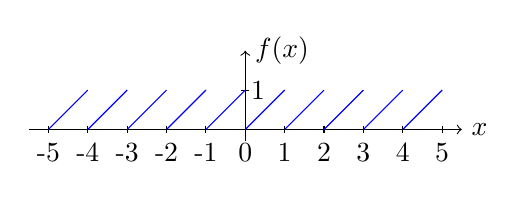
\begin{tikzpicture}[scale=0.5]
    % Axis
    \draw[->] (-5.5,0) -- (5.5,0) node[right] {\( x \)};
    \draw[->] (0,-0.3) -- (0,2) node[right] {\( f(x) \)};
    
    % Ticks
    \foreach \x in {-5,-4,...,5} {
        \draw (\x, 0.1) -- (\x, -0.1) node[below] {\x};
    }

    
    \draw (0.1, 1) -- (-0.1, 1) node[right] {1};
    
    % Function plot
    \foreach \n in {-5,-4,...,4} {
        \draw[blue] (\n, 0) -- (\n+1, 1);
    }
\end{tikzpicture}
\caption{$f(x)=x-[x]$的图像}
\label{fig:f(x)=x-[x]的图像}
\end{figure}

\item 常量函数 $f(x)=c$ 是以任何正数为周期的周期函数,但不存在基本周期.
        \end{enumerate}
\end{exercise}

\subsection{初等函数}

我们在中学接触过的基本初等函数有如表\ref{tab:基本初等函数分类表}所示的六类。它们的函数图像如图\ref{fig:basic-elem-func}所示。

\begin{table}[h]
\caption{基本初等函数分类表}
\centering
\renewcommand{\arraystretch}{1.5} % 用于增加行高
\begin{tabular}{c|c}
\hline
\rowcolor{gray!50}
\textbf{函数类型} & \textbf{函数表达式} \\
\hline
常量函数 & $y=c \quad (c$ 是常数$)$ \\
\hline
幂函数 & $y=x^u \quad (u$ 为实数$)$ \\
\hline
指数函数 & $y=a^x \quad (a>0, a \neq 1)$ \\
\hline
对数函数 & $y=\log_a x \quad (a>0, a \neq 1)$ \\
\hline
\multirow{4}{*}{三角函数} & $y=\sin x$ (正弦函数) \\
 & $y=\cos x$ (余弦函数) \\
 & $y=\tan x$ (正切函数) \\
 & $y=\cot x$ (余切函数) \\
\hline
\multirow{4}{*}{反三角函数} & $y=\arcsin x$ (反正弦函数) \\
 & $y=\arccos x$ (反余弦函数) \\
 & $y=\arctan x$ (反正切函数) \\
 & $y=\operatorname{arccot} x$ (反余切函数) \\
\hline
\end{tabular}
\label{tab:基本初等函数分类表}
\end{table}

\begin{figure}[!h]
    \centering
\begin{tikzpicture}[scale=0.8]

  % Draw axes
  \draw[->, thick] (-6,0) -- (6,0) node[right] {$x$};
  \draw[->, thick] (0,-6) -- (0,6) node[above] {$y$};
  
  % Draw grid
  \draw[gray!50, very thin] (-5.9,-5.9) grid[step=1cm] (5.9,5.9);
  
  % Plot constant function f(x) = 1
  \draw[myred, thick, domain=-5:5, samples=2] plot (\x, {1}) node[right] {$f(x)=1$};
  
  % Plot linear function f(x) = x
  \draw[myblue, thick, domain=-4.7:4.7, samples=2] plot (\x, {\x}) node[right] {$f(x)=x$};
  
  % Plot quadratic function f(x) = x^2
  \draw[mygreen, thick, domain=-2.25:2.25, samples=50] plot (\x, {\x*\x}) node[right] {$f(x)=x^2$};

  % Plot quadratic function f(x) = x^3
  \draw[mypurple, thick, domain=-1.7:1.7, samples=50] plot (\x, {\x*\x*\x}) node[left] {$f(x)=x^3$};
  
  % Plot exponential function f(x) = e^x
  \draw[myorange, thick, domain=-2:1.75, samples=50] plot (\x, {exp(\x)}) node[right] {$f(x)=e^x$};
  
  % Plot logarithmic function f(x) = ln(x)
  \draw[mybrown, thick, domain=0.1:5, samples=50] plot (\x, {ln(\x)}) node[right] {$f(x)=\ln(x)$};

  % Mark points
  % \filldraw [black] (1,0) circle (2pt) node[anchor=north west] {(1, 0)};
  \filldraw [black] (0,0) circle (2pt) node[anchor=north west] {(0, 0)};
  % \filldraw [black] (0,1) circle (2pt) node[anchor=north east] {(0, 1)};
  \filldraw [black] (1,1) circle (2pt) node[anchor=south west] {(1, 1)};

\end{tikzpicture}
\caption{基本初等函数的图像}
    \label{fig:basic-elem-func}
\end{figure}

幂函数 $y=x^u$ 和指数函数 $y=a^x$ 都涉及乘幂, 而在中学数 课程中只给出了有理指数乘幂的定义. 这里我们指出,无理数也可以作为幂指数。\textcolor{second}{无理指数幂和有理指数幂一起构成了实数指数幂,并保持有理指数幂的基本性质。}


\begin{definition}[初等函数]
    由基本初等函数经过\textcolor{red}{有限次四则运算与复合运算}所得到的函数, 统称为\textcolor{third}{\bf 初等函数}.
\end{definition}


\subsection{复合函数}

\subsection{反函数}